\documentclass[aspectratio=169]{beamer}

% ── Theme & Colors ──────────────────────────────────────────────────────────
\usetheme{Madrid}
\usecolortheme{default}

\definecolor{fptblue}{RGB}{30, 58, 138}
\definecolor{fptaccent}{RGB}{221, 132, 82}
\definecolor{fptgood}{RGB}{85, 168, 104}
\definecolor{fptbad}{RGB}{196, 78, 82}

\setbeamercolor{palette primary}{bg=fptblue, fg=white}
\setbeamercolor{palette secondary}{bg=fptblue!80, fg=white}
\setbeamercolor{palette tertiary}{bg=fptblue!60, fg=white}
\setbeamercolor{structure}{fg=fptblue}
\setbeamercolor{title}{fg=white, bg=fptblue}
\setbeamercolor{frametitle}{fg=white, bg=fptblue}
\setbeamercolor{block title}{bg=fptblue, fg=white}
\setbeamercolor{block body}{bg=fptblue!5}
\setbeamercolor{item}{fg=fptblue}
\setbeamercolor{alerted text}{fg=fptbad}

\setbeamertemplate{navigation symbols}{}
\setbeamertemplate{footline}{%
  \leavevmode\hbox{%
    \begin{beamercolorbox}[wd=.333\paperwidth,ht=2.5ex,dp=1ex,center]{palette primary}%
      \usebeamerfont{author in head/foot}\insertshortauthor
    \end{beamercolorbox}%
    \begin{beamercolorbox}[wd=.334\paperwidth,ht=2.5ex,dp=1ex,center]{palette secondary}%
      \usebeamerfont{title in head/foot}\insertshorttitle
    \end{beamercolorbox}%
    \begin{beamercolorbox}[wd=.333\paperwidth,ht=2.5ex,dp=1ex,right]{palette tertiary}%
      \insertframenumber{} / \inserttotalframenumber\hspace*{2ex}
    \end{beamercolorbox}%
  }%
}

% ── Packages ────────────────────────────────────────────────────────────────
\usepackage{graphicx}
\usepackage{booktabs}
\usepackage{amsmath}
\usepackage{hyperref}
\usepackage{colortbl}
\graphicspath{{figures/}}

% ── Title ───────────────────────────────────────────────────────────────────
\title[EV Price Prediction]{Electric Vehicle Price Prediction\\in the Vietnamese Market}
\subtitle{A Web-Scraped Dataset with LLM-Assisted Feature Extraction}
\author[Hoang et al.]{Anh~D.~D.~Hoang \and Khang~H.~Tran \and Anh~N.~Vu \and Nam~N.~Trinh}
\institute[FPT University]{%
  Information Technology Specialization\\
  FPT University, Hanoi, Vietnam
}
\date{AIL301m --- March 2026}
\titlegraphic{
\includegraphics[height=1.2cm]{FPT_logo}}

\begin{document}

% ════════════════════════════════════════════════════════════════════════════
\begin{frame}
  \titlepage
\end{frame}

% ════════════════════════════════════════════════════════════════════════════
\begin{frame}{Outline}
  \tableofcontents
\end{frame}

% ════════════════════════════════════════════════════════════════════════════
\section{Introduction}

\begin{frame}{Motivation}
  \begin{columns}[T]
    \begin{column}{0.55\textwidth}
      \begin{itemize}
        \item Vietnam's EV market is \textbf{growing rapidly}
          \begin{itemize}
            \item VinFast mass-producing since 2022
            \item Chinese imports (BYD, Wuling, Geely)
            \item Government ICE phase-out by 2040
          \end{itemize}
        \item \textbf{No structured dataset} exists for Vietnamese EV prices
        \item No local equivalent of Kelley Blue Book or AutoTrader
        \item Listings are \textbf{unstructured, Vietnamese-language}, scattered across multiple platforms
      \end{itemize}
    \end{column}
    \begin{column}{0.42\textwidth}
      \begin{block}{Gap}
        Existing car price prediction studies rely on clean, single-source, Western-market datasets
      \end{block}
      \vspace{0.5em}
      \begin{block}{Our Goal}
        End-to-end pipeline: \textbf{scraping $\to$ LLM extraction $\to$ data quality $\to$ prediction}
      \end{block}
    \end{column}
  \end{columns}
\end{frame}

\begin{frame}{Contributions}
  \begin{enumerate}
    \item \textbf{First Vietnamese EV dataset} --- 4,166 records from 4 marketplaces with unified 20-column schema
    \item \textbf{Two-stage LLM extraction} --- local Qwen 2.5 3B + cloud GPT-5-nano with auto-retry and Pydantic validation
    \item \textbf{Data quality analysis} --- identified and corrected 3 critical issues, reducing RMSE by \textbf{67\%} (1.02B $\to$ 332M VND)
    \item \textbf{Segment-specific evaluation} --- practical accuracy (RMSE $< 100$M) for budget \& mid-range segments (56\% of market)
  \end{enumerate}

  \vspace{1em}
  \begin{alertblock}{Key Finding}
    Data quality remediation contributes \textbf{far more} to accuracy than model selection (67\% vs 15\% RMSE improvement).
  \end{alertblock}
\end{frame}

% ════════════════════════════════════════════════════════════════════════════
\section{Data Collection}

\begin{frame}{Data Sources}
  \begin{columns}[T]
    \begin{column}{0.55\textwidth}
      \begin{table}
        \centering
        \small
        \begin{tabular}{llr}
          \toprule
          \textbf{Website} & \textbf{Method} & \textbf{Records} \\
          \midrule
          bonbanh.com      & BeautifulSoup & 1,502 \\
          chotot.com       & Scrapy        & 1,727 \\
          xevinfastluot.com & Selenium     & 208 \\
          otodien.vn       & BeautifulSoup & 729 \\
          \midrule
          \textbf{Total}   &               & \textbf{4,166} \\
          \bottomrule
        \end{tabular}
      \end{table}
      \vspace{0.5em}
      \small
      Unified schema: 20 columns covering ID, specs, condition, metadata, and price
    \end{column}
    \begin{column}{0.42\textwidth}
      \begin{figure}
        \centering
        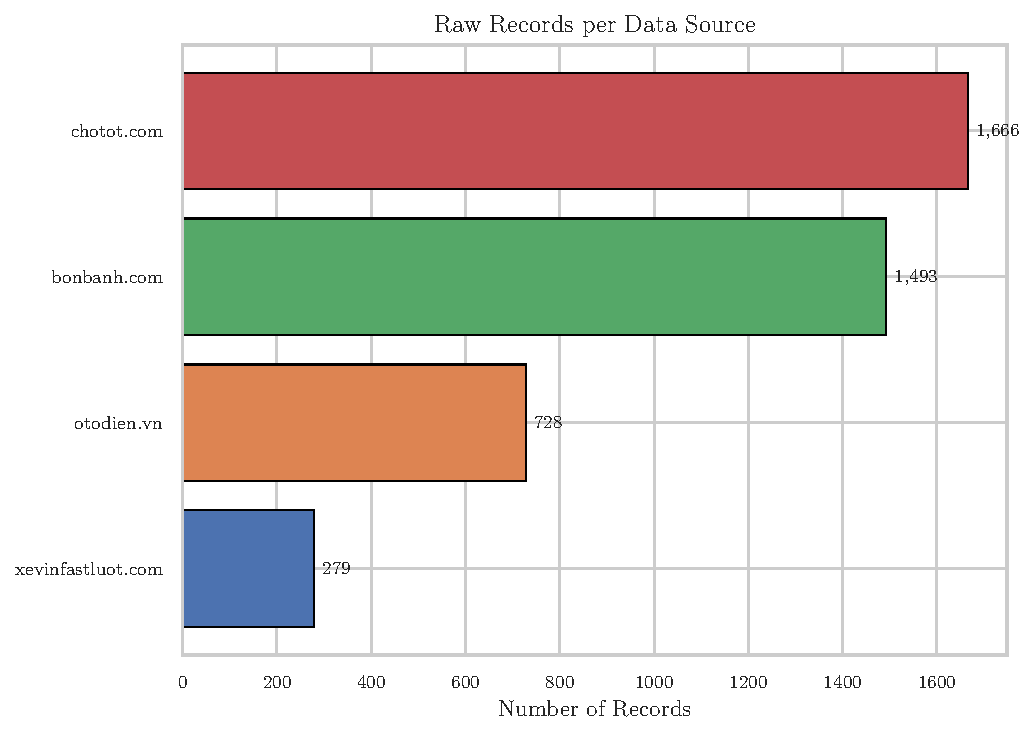
\includegraphics[width=\textwidth]{records_per_source}
        \caption{Records per source}
      \end{figure}
    \end{column}
  \end{columns}
\end{frame}

\begin{frame}{LLM-Assisted Feature Extraction}
  \begin{block}{Two-Stage Pipeline}
    \begin{enumerate}
      \item \textbf{Local --- Qwen 2.5 3B} (via Ollama)
        \begin{itemize}
          \item Zero-shot prompt $\to$ JSON output
          \item Pydantic schema validation
          \item Auto-retry up to 3 attempts on failure
        \end{itemize}
      \item \textbf{Cloud --- GPT-5-nano} (verification)
        \begin{itemize}
          \item Batch-processes low-confidence records
          \item Corrects hallucinated trim names
        \end{itemize}
    \end{enumerate}
  \end{block}

  \vspace{0.5em}
  \begin{columns}[T]
    \begin{column}{0.45\textwidth}
      \textbf{Fill rates:}\\[0.3em]
      \small
      Brand: 99.3\% \quad Base model: 98.7\%\\
      Year: 98.3\% \quad Price: 100\%
    \end{column}
    \begin{column}{0.45\textwidth}
      \textbf{Failure mode:}\\[0.3em]
      \small
      Trim-level hallucination for non-VinFast brands
    \end{column}
  \end{columns}
\end{frame}

% ════════════════════════════════════════════════════════════════════════════
\section{Data Quality Analysis}

\begin{frame}{Three Critical Issues}
  \begin{columns}[T]
    \begin{column}{0.32\textwidth}
      \begin{block}{\small 1. chotot.com 10$\times$ Inflation}
        \small
        \begin{itemize}
          \item 1,727 records (41\%)
          \item Unit mismatch in LLM extraction
          \item Fix: divide by 10
        \end{itemize}
      \end{block}
    \end{column}
    \begin{column}{0.32\textwidth}
      \begin{block}{\small 2. BYD Pricing Error}
        \small
        \begin{itemize}
          \item 74 records (2.3\%)
          \item 14.5\% of total MAE
          \item Fix: remove all BYD
        \end{itemize}
      \end{block}
    \end{column}
    \begin{column}{0.32\textwidth}
      \begin{block}{\small 3. Duplicate Leakage}
        \small
        \begin{itemize}
          \item 883 duplicates (22\%)
          \item Inflated $R^2$: 0.787
          \item Honest $R^2$: 0.725
        \end{itemize}
      \end{block}
    \end{column}
  \end{columns}

  \vspace{1em}
  \centering
  \begin{tabular}{lrr}
    \toprule
    \textbf{Stage} & \textbf{Records} & \textbf{Best RMSE} \\
    \midrule
    Raw (all issues) & 3,963 & 1.02B VND \\
    + All fixes applied & 3,015 & \textbf{332M VND} \\
    \bottomrule
  \end{tabular}
  \quad \textcolor{fptgood}{\textbf{$\downarrow$ 67\% RMSE reduction}}
\end{frame}

\begin{frame}{chotot.com Price Inflation}
  \begin{figure}
    \centering
    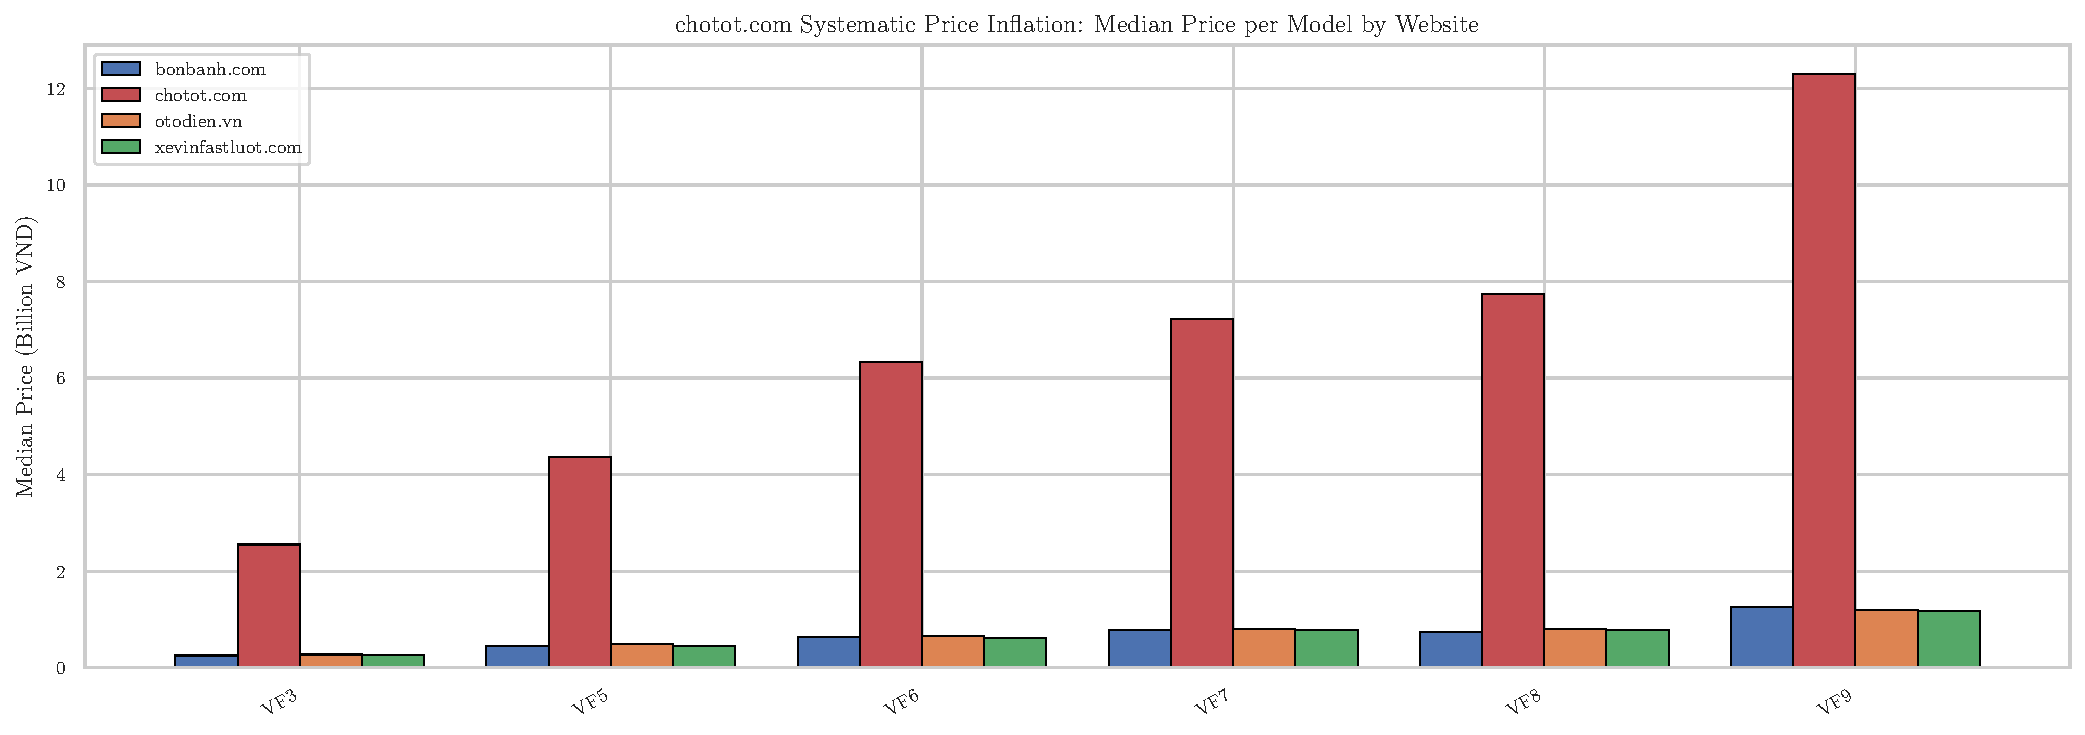
\includegraphics[width=0.85\textwidth]{chotot_price_comparison}
    \caption{Systematic 10$\times$ price inflation from chotot.com vs other sources}
  \end{figure}
\end{frame}

\begin{frame}{Before vs After Data Quality Fixes}
  \begin{figure}
    \centering
    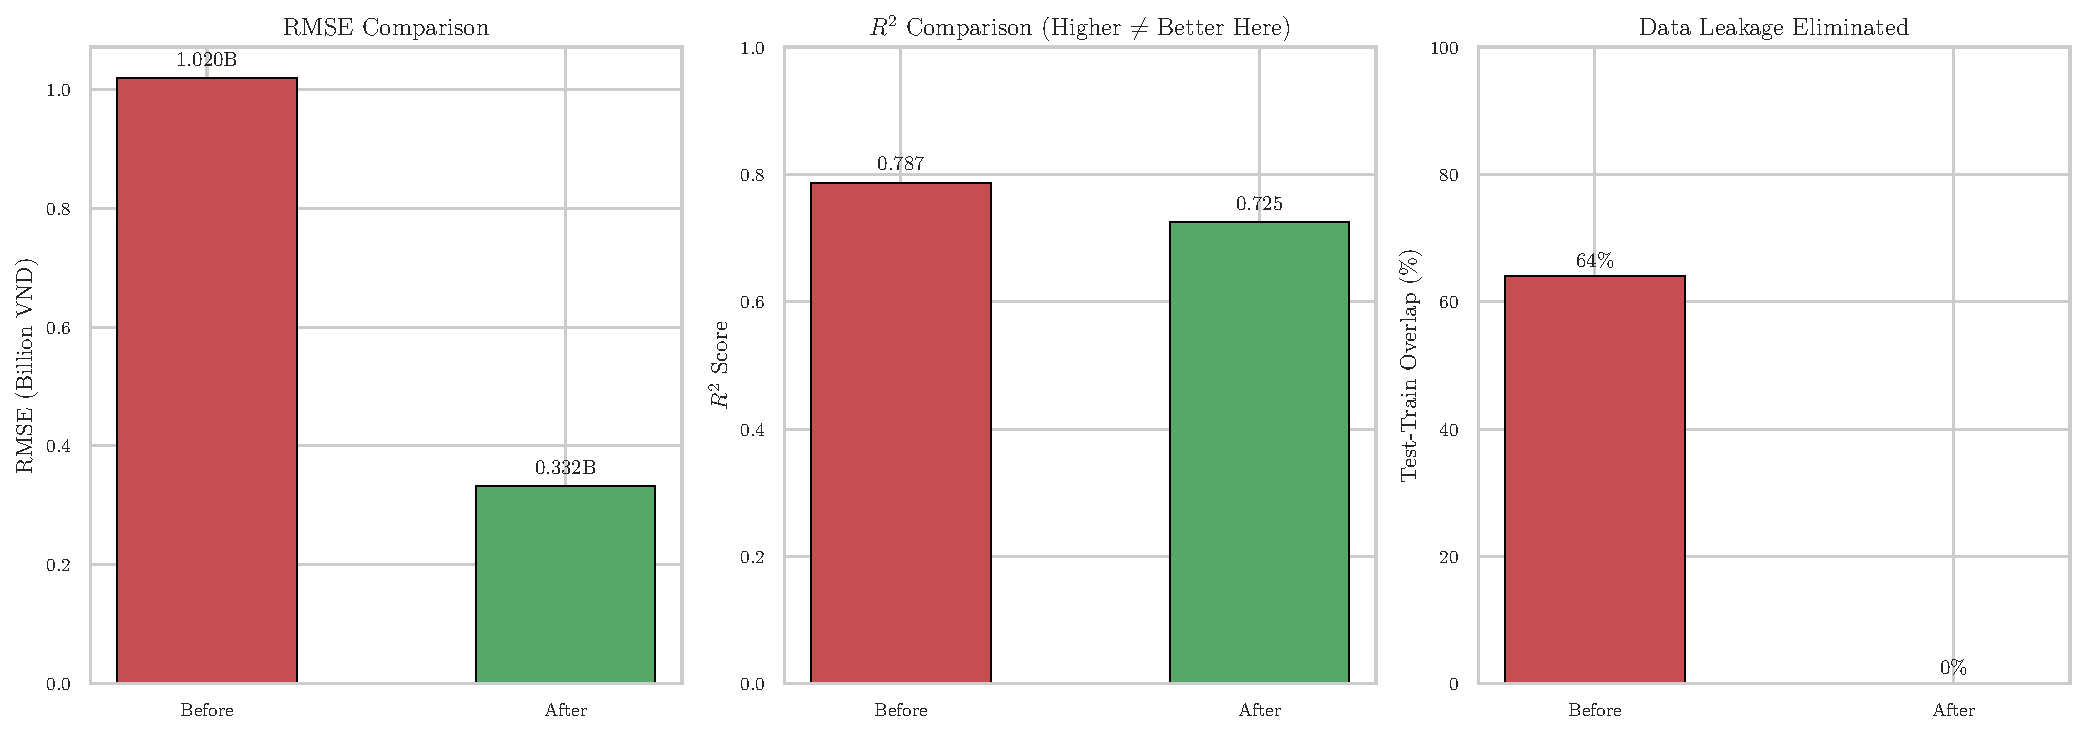
\includegraphics[width=0.85\textwidth]{before_after_comparison}
    \caption{Model performance before and after corrections --- ``before'' metrics were inflated by leakage}
  \end{figure}
\end{frame}

% ════════════════════════════════════════════════════════════════════════════
\section{Feature Engineering}

\begin{frame}{Feature Engineering Pipeline}
  \begin{columns}[T]
    \begin{column}{0.48\textwidth}
      \textbf{41 features} from 3,015 records:
      \vspace{0.5em}
      \small
      \begin{tabular}{lr}
        \toprule
        \textbf{Category} & \textbf{Count} \\
        \midrule
        Numeric (age, mileage, \ldots) & 4 \\
        EV Specs (kWh, range, hp) & 3 \\
        Target-encoded & 2 \\
        One-hot (brand, model, \ldots) & 32 \\
        \midrule
        \textbf{Total} & \textbf{41} \\
        \bottomrule
      \end{tabular}
    \end{column}
    \begin{column}{0.48\textwidth}
      \begin{block}{Key Decisions}
        \begin{itemize}
          \small
          \item \textbf{EV specs recovery}: battery, range, power from otodien.vn lookup (29 models)
          \item \textbf{Hybrid encoding}: target-encode only high-cardinality features
          \item Target-encoding everything $\Rightarrow$ $R^2$ drops to 0.087!
        \end{itemize}
      \end{block}
    \end{column}
  \end{columns}
\end{frame}

\begin{frame}{EV Specifications Recovery}
  \begin{figure}
    \centering
    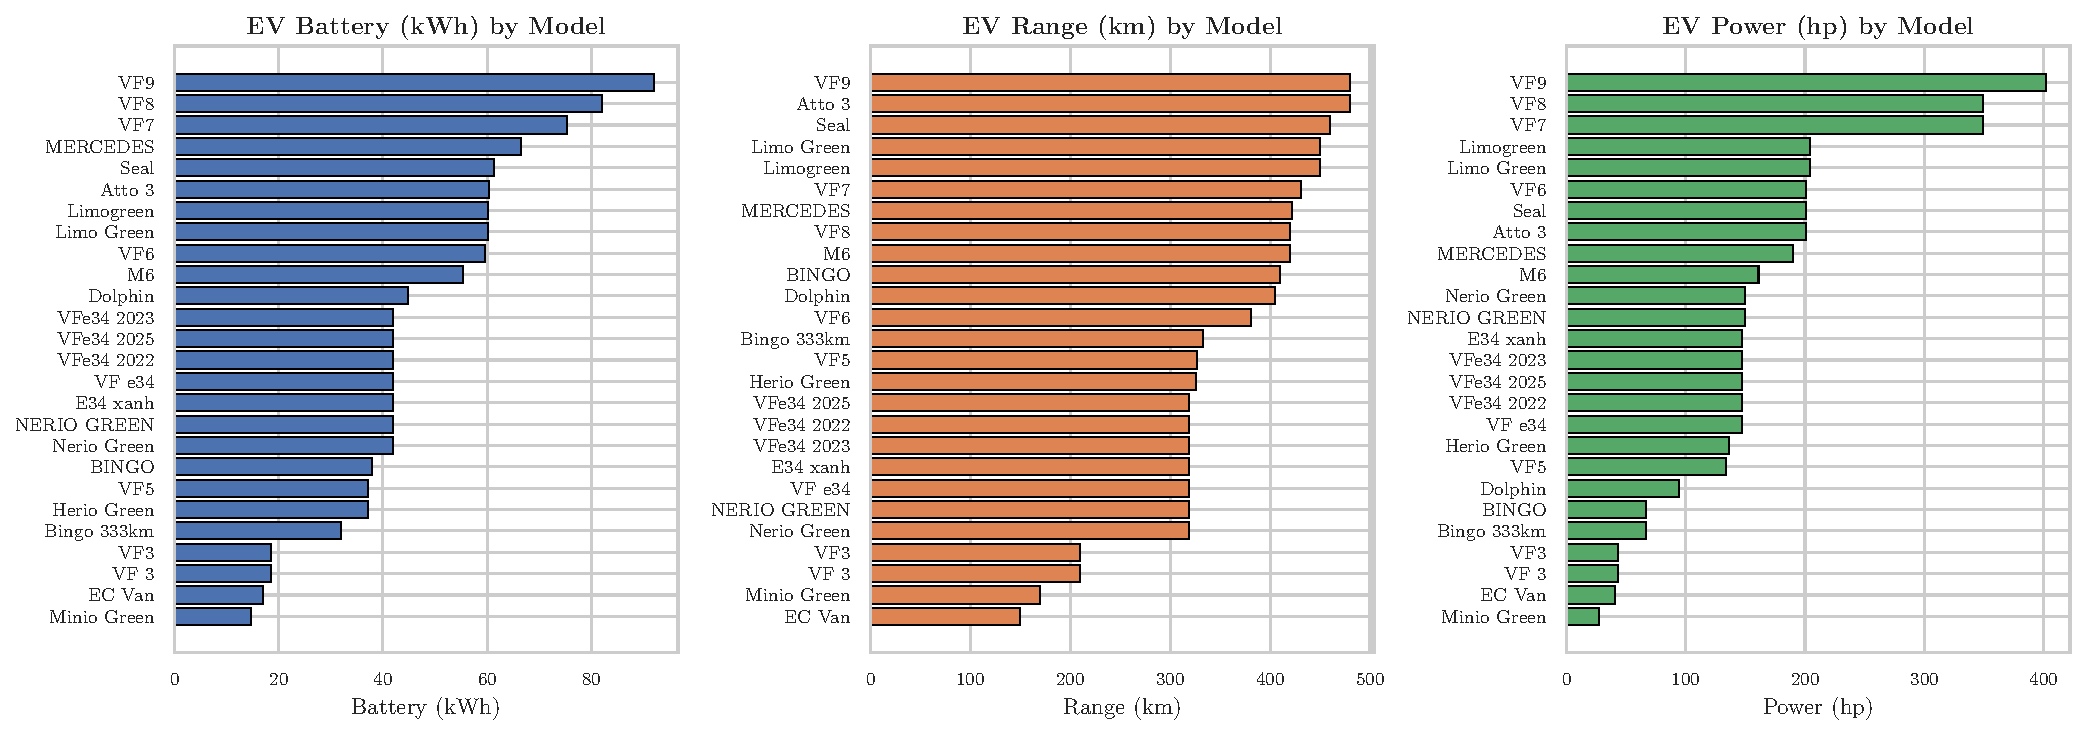
\includegraphics[width=0.85\textwidth]{ev_specs_coverage}
    \caption{EV specifications across models --- captures fundamental pricing physics}
  \end{figure}
\end{frame}

\begin{frame}{Encoding Strategy \& Feature Importance}
  \begin{columns}[T]
    \begin{column}{0.45\textwidth}
      \begin{figure}
        \centering
        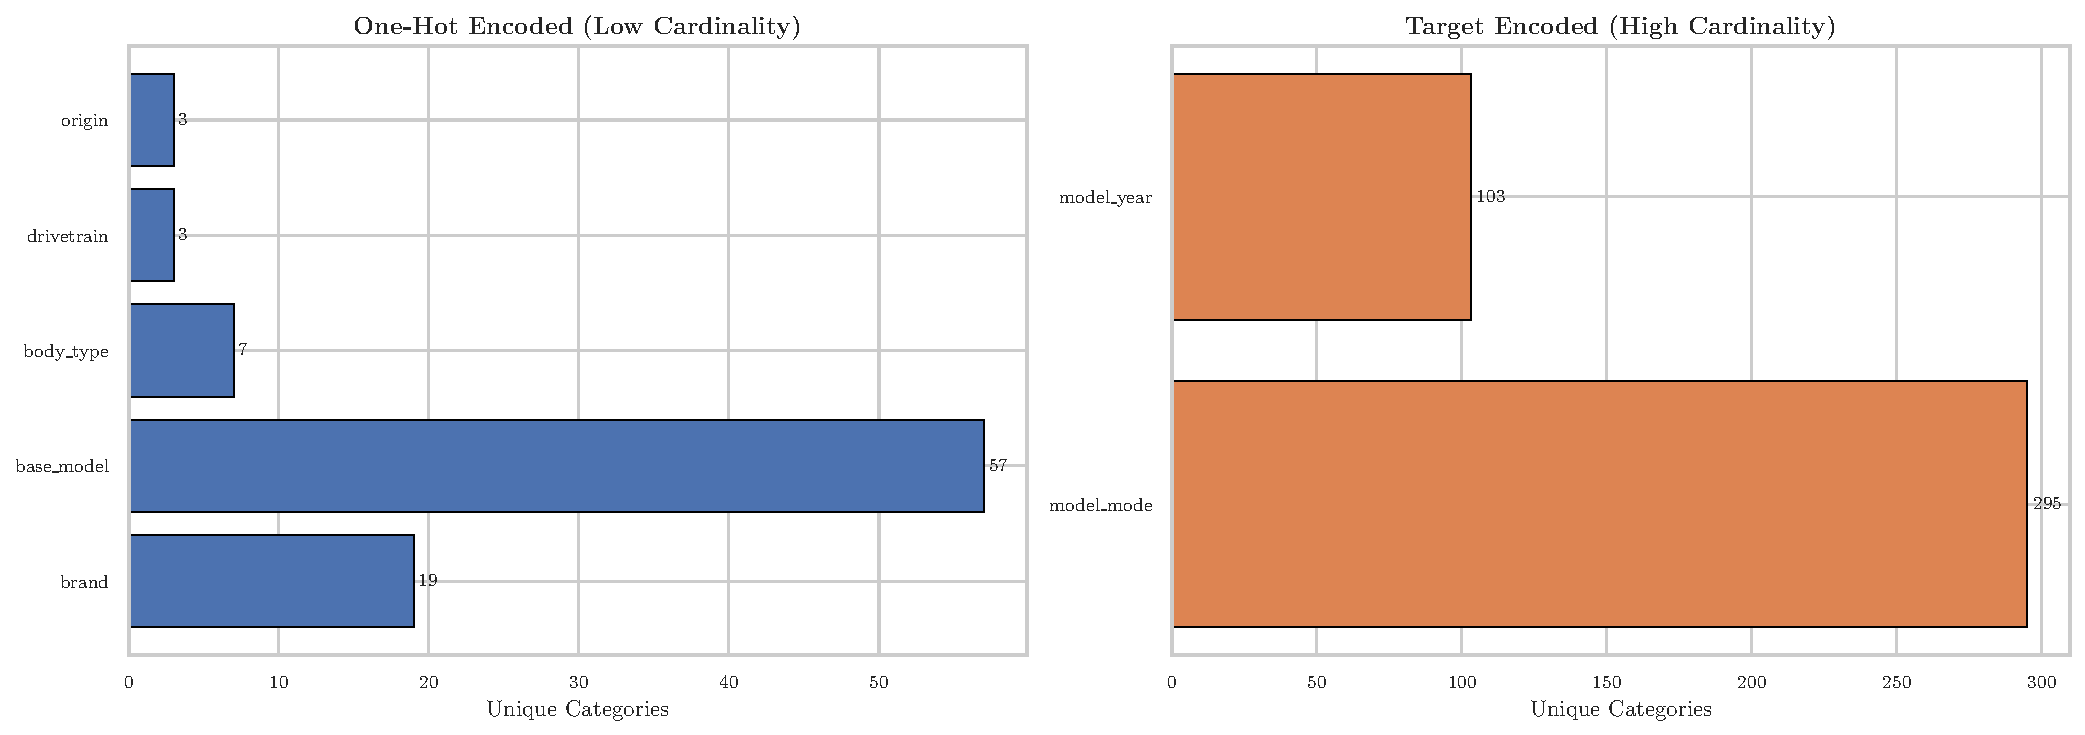
\includegraphics[width=\textwidth]{encoding_comparison}
        \caption{Hybrid encoding}
      \end{figure}
    \end{column}
    \begin{column}{0.52\textwidth}
      \begin{figure}
        \centering
        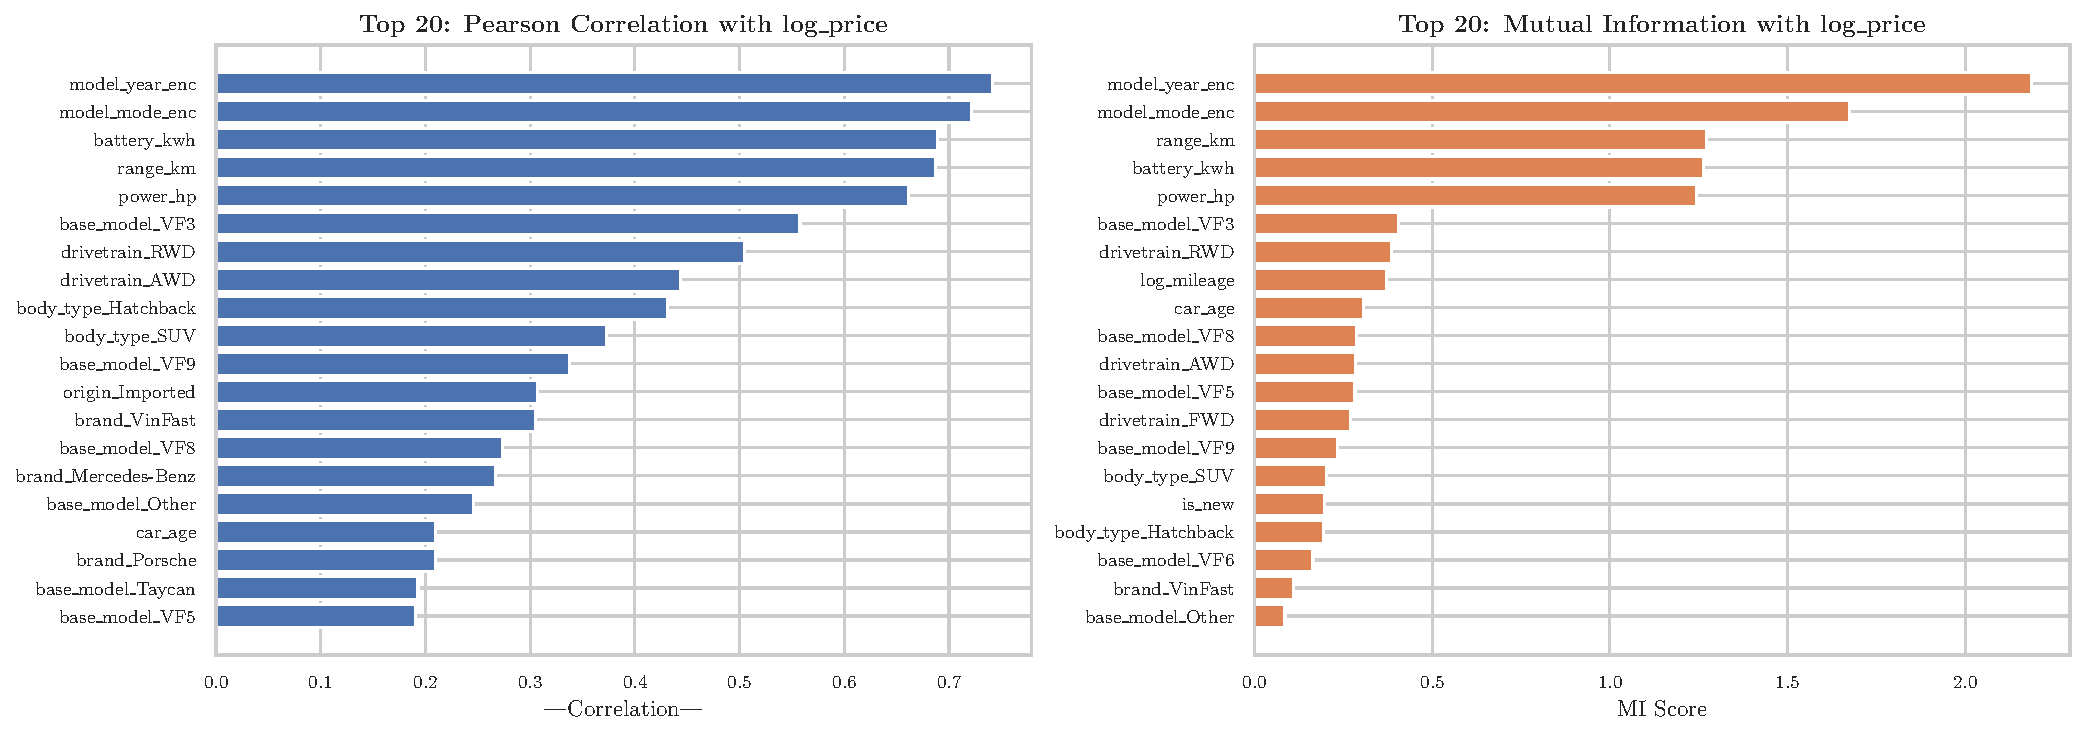
\includegraphics[width=\textwidth]{feature_importance_summary}
        \caption{Top features by correlation \& MI}
      \end{figure}
    \end{column}
  \end{columns}
\end{frame}

% ════════════════════════════════════════════════════════════════════════════
\section{Experimental Setup}

\begin{frame}{Experimental Setup}
  \begin{columns}[T]
    \begin{column}{0.48\textwidth}
      \textbf{Data Split:}
      \begin{itemize}
        \item 80/20 train--test (2,412 / 603)
        \item Stratified on \texttt{base\_model}
        \item Sample weights: inverse quintile frequency
      \end{itemize}

      \vspace{1em}
      \textbf{Evaluation:}
      \begin{itemize}
        \item RMSE, MAE, $R^2$, Adj.\ $R^2$, MAPE
        \item 95\% CI via bootstrap (1,000 resamples)
        \item Segment-specific analysis
      \end{itemize}
    \end{column}
    \begin{column}{0.48\textwidth}
      \textbf{Four Models:}
      \vspace{0.5em}
      \small
      \begin{tabular}{ll}
        \toprule
        \textbf{Model} & \textbf{Input} \\
        \midrule
        Ridge & Scaled + log target \\
        SVR (RBF) & Scaled + log target \\
        Random Forest & Raw features \\
        XGBoost & Raw features \\
        \bottomrule
      \end{tabular}

      \vspace{1em}
      \normalsize
      All tuned via \textbf{5-fold CV} with GridSearchCV
    \end{column}
  \end{columns}
\end{frame}

% ════════════════════════════════════════════════════════════════════════════
\section{Results}

\begin{frame}{Overall Benchmark}
  \begin{table}
    \centering
    \begin{tabular}{lrrrrr}
      \toprule
      \textbf{Model} & \textbf{RMSE} & \textbf{MAE} & $\boldsymbol{R^2}$ & \textbf{Adj.\ $R^2$} & \textbf{MAPE} \\
       & (M VND) & (M VND) & & & (\%) \\
      \midrule
      Ridge & 381 & 115 & 0.636 & 0.610 & 43.5 \\
      SVR & 369 & 94 & 0.660 & 0.635 & 48.9 \\
      \rowcolor{fptblue!10} \textbf{Random Forest} & \textbf{332} & \textbf{89} & \textbf{0.725} & \textbf{0.705} & \textbf{43.6} \\
      XGBoost & 383 & 103 & 0.633 & 0.606 & 43.0 \\
      \bottomrule
    \end{tabular}
    \caption{Test set results ($n = 603$). RF 95\% CI for RMSE: [139M, 496M] VND.}
  \end{table}

  \vspace{0.5em}
  \centering
  \textcolor{fptblue}{\textbf{Random Forest wins across all metrics}}
\end{frame}

\begin{frame}{Model Comparison}
  \begin{columns}[c]
    \begin{column}{0.48\textwidth}
      \begin{figure}
        \centering
        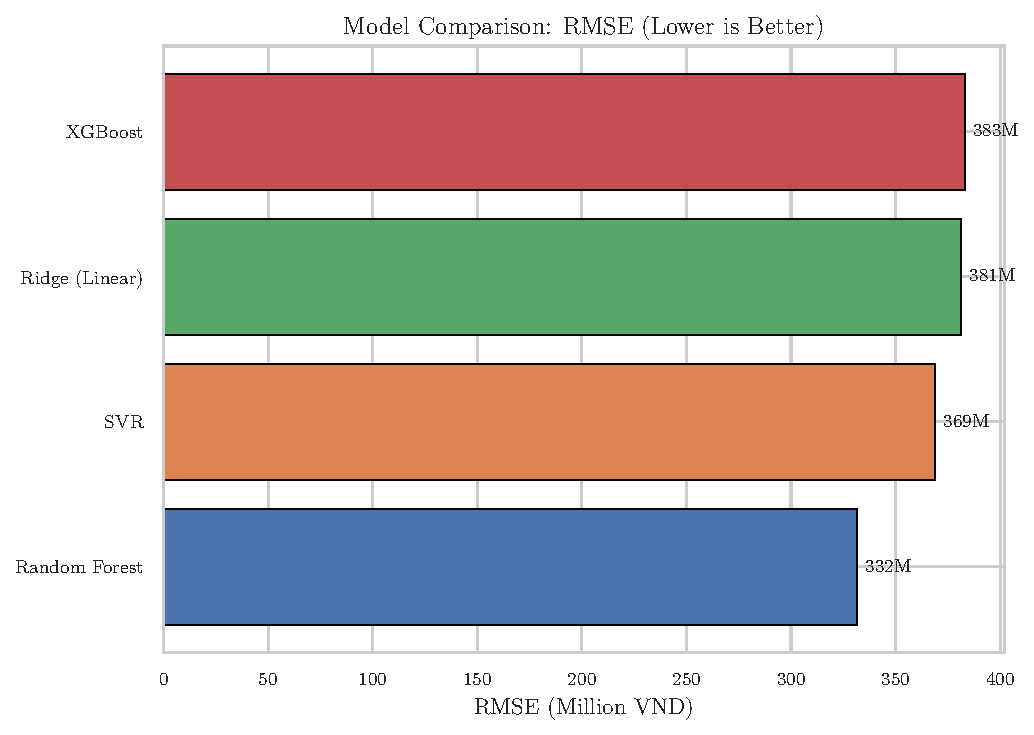
\includegraphics[width=\textwidth]{model_rmse_comparison}
        \caption{RMSE comparison}
      \end{figure}
    \end{column}
    \begin{column}{0.48\textwidth}
      \begin{figure}
        \centering
        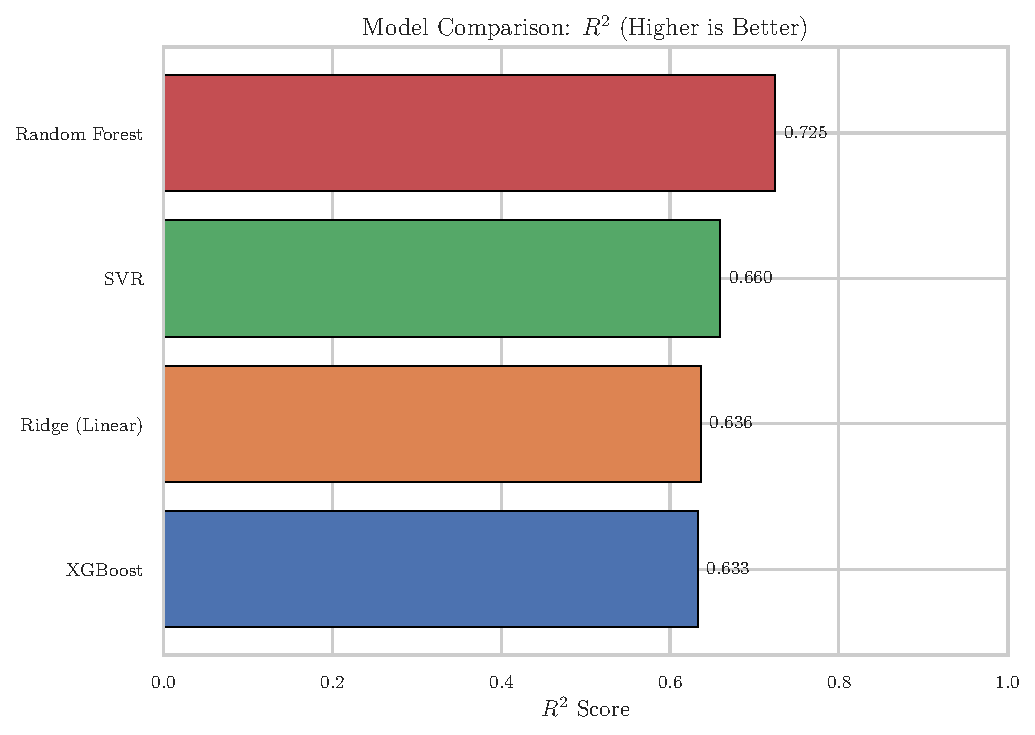
\includegraphics[width=\textwidth]{model_r2_comparison}
        \caption{$R^2$ comparison}
      \end{figure}
    \end{column}
  \end{columns}
\end{frame}

\begin{frame}{Segment-Specific Performance}
  \begin{columns}[T]
    \begin{column}{0.45\textwidth}
      \begin{table}
        \centering
        \small
        \begin{tabular}{lrr}
          \toprule
          \textbf{Segment} & \textbf{RMSE} & $\boldsymbol{n}$ \\
          \midrule
          Budget ($<$500M) & \textcolor{fptgood}{100M} & 237 \\
          Mid (0.5--1.2B) & \textcolor{fptgood}{81M} & 318 \\
          Premium (1.2--5B) & \textcolor{fptaccent}{797M} & 46 \\
          Luxury ($>$5B) & \textcolor{fptbad}{4,041M} & 2 \\
          \midrule
          \textbf{Overall} & \textbf{332M} & 603 \\
          \bottomrule
        \end{tabular}
        \caption{RF by segment}
      \end{table}
      \vspace{0.3em}
      \small
      Budget + Mid = \textbf{92\% of test data} with practical RMSE
    \end{column}
    \begin{column}{0.52\textwidth}
      \begin{figure}
        \centering
        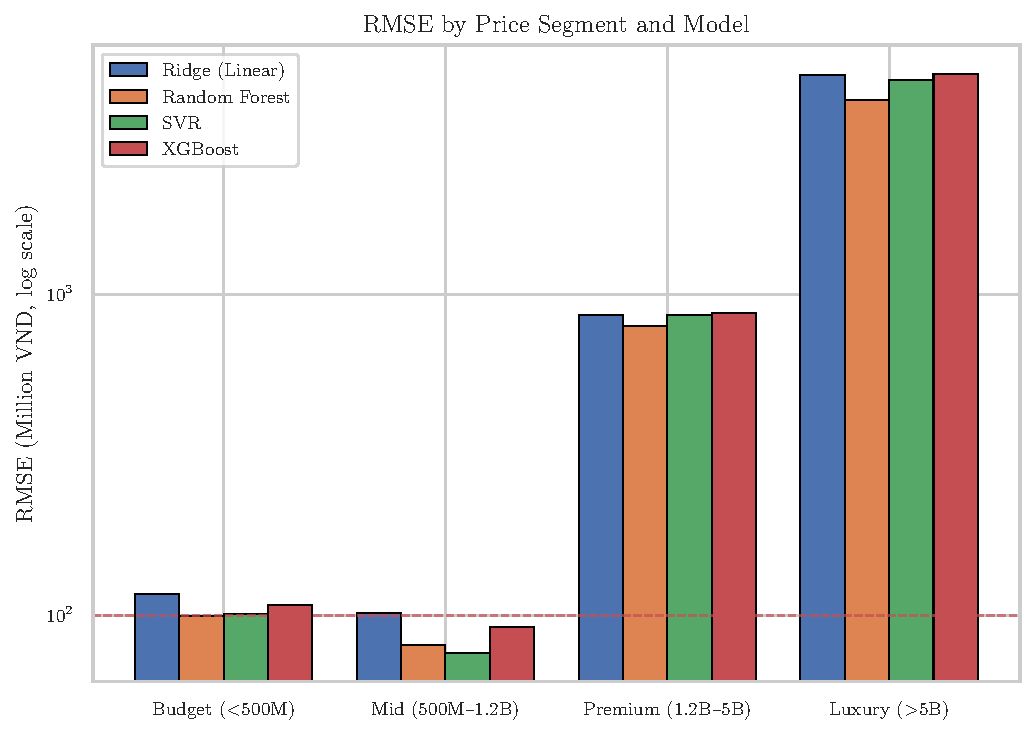
\includegraphics[width=\textwidth]{segment_rmse}
        \caption{RMSE by segment (all models)}
      \end{figure}
    \end{column}
  \end{columns}
\end{frame}

\begin{frame}{Random Forest: Predictions \& Feature Importance}
  \begin{columns}[c]
    \begin{column}{0.48\textwidth}
      \begin{figure}
        \centering
        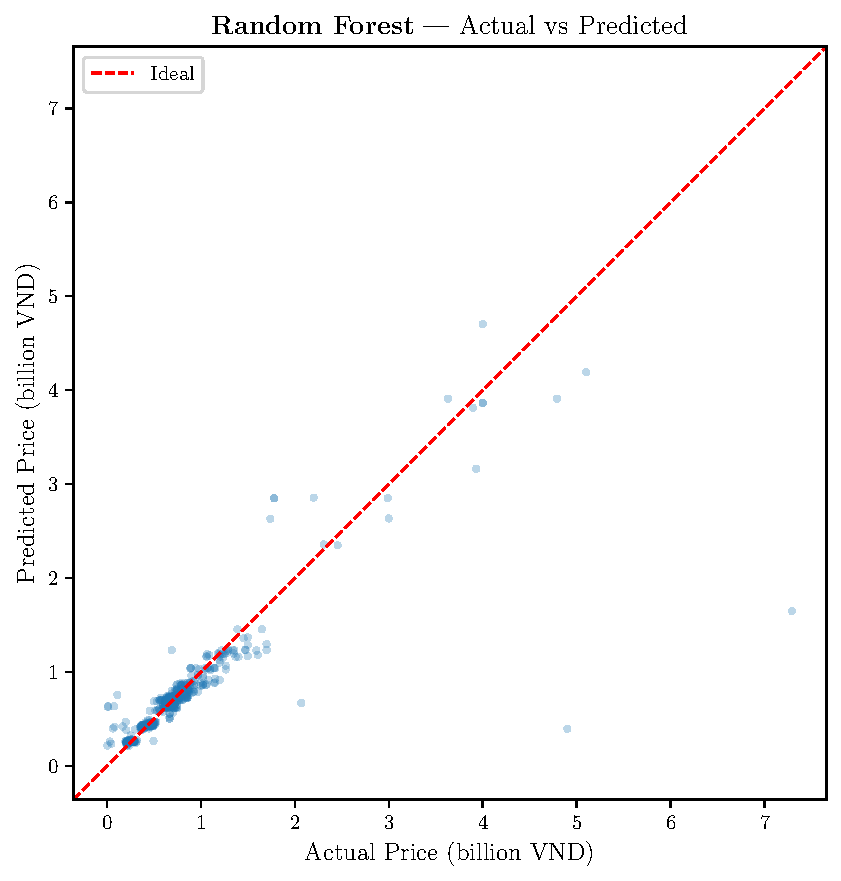
\includegraphics[width=\textwidth]{random_forest_actual_vs_predicted}
        \caption{Actual vs Predicted}
      \end{figure}
    \end{column}
    \begin{column}{0.48\textwidth}
      \begin{figure}
        \centering
        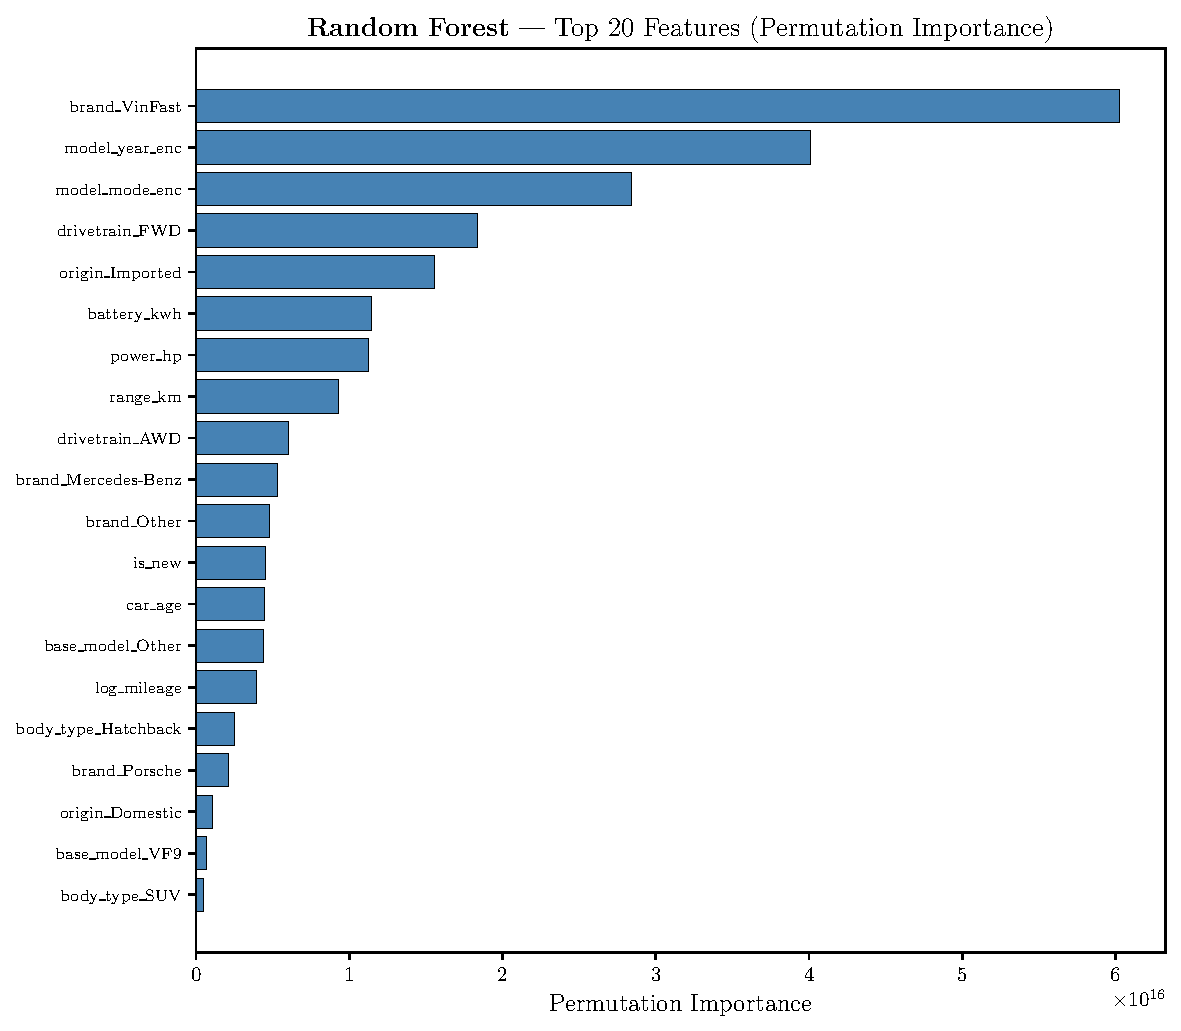
\includegraphics[width=\textwidth]{random_forest_feature_importance}
        \caption{Top 20 feature importance}
      \end{figure}
    \end{column}
  \end{columns}
\end{frame}

% ════════════════════════════════════════════════════════════════════════════
\section{Discussion \& Conclusion}

\begin{frame}{Data Quality vs Model Selection}
  \begin{columns}[T]
    \begin{column}{0.48\textwidth}
      \begin{block}{Data Quality Fixes}
        RMSE: 1.02B $\to$ 332M VND\\
        \textcolor{fptgood}{\textbf{$\downarrow$ 67\% improvement}}
        \begin{itemize}
          \small
          \item chotot.com price correction
          \item Deduplication (22\% removed)
          \item BYD removal
        \end{itemize}
      \end{block}
    \end{column}
    \begin{column}{0.48\textwidth}
      \begin{block}{Model Selection}
        Best vs Worst: 332M vs 383M\\
        \textcolor{fptaccent}{\textbf{$\downarrow$ 15\% difference}}
        \begin{itemize}
          \small
          \item RF vs XGBoost: 51M gap
          \item All models benefit equally from clean data
        \end{itemize}
      \end{block}
    \end{column}
  \end{columns}

  \vspace{1em}
  \begin{alertblock}{Takeaway}
    In applied ML with web-scraped data, \textbf{invest in data quality first} --- it yields 4$\times$ more improvement than model experimentation.
  \end{alertblock}
\end{frame}

\begin{frame}{Limitations \& Future Work}
  \textbf{Limitations:}
  \begin{itemize}
    \item \textbf{Brand concentration} --- VinFast = 93.6\% of records
    \item \textbf{Small dataset} --- 3,015 records (2,412 train)
    \item \textbf{No temporal modeling} --- cross-sectional only
    \item \textbf{Luxury segment} --- only 2 test records ($n$ too small)
  \end{itemize}

  \vspace{1em}
  \textbf{Future Work:}
  \begin{enumerate}
    \item Continuous scraping $\to$ time-series depreciation model
    \item Additional sources (dealer prices, registration data)
    \item Ensemble stacking of all four models
    \item Expand to hybrid \& plug-in hybrid vehicles
  \end{enumerate}
\end{frame}

\begin{frame}{Conclusion}
  \begin{block}{Summary}
    \begin{itemize}
      \item End-to-end pipeline: \textbf{scraping $\to$ LLM extraction $\to$ data quality $\to$ feature engineering $\to$ prediction}
      \item Data quality fixes reduced RMSE by \textbf{67\%} (1.02B $\to$ 332M VND)
      \item Random Forest: $R^2 = 0.725$, RMSE = 332M VND
      \item \textbf{Practical accuracy} for budget + mid segments (56\% of market, RMSE $\leq$ 100M)
    \end{itemize}
  \end{block}

  \vspace{1em}
  \centering
  \large
  \textcolor{fptblue}{\textbf{Data quality $>$ Model selection}}\\[0.5em]
  \small
  In real-world ML with scraped data, the dominant bottleneck is data quality, not model architecture.
\end{frame}

\begin{frame}{}
  \centering
  \vfill
  {\Huge\textcolor{fptblue}{\textbf{Thank You}}}\\[1.5em]
  {\large Questions?}\\[2em]
  
\includegraphics[height=1.5cm]{FPT_logo}\\[1em]
  \small
  Anh D.D. Hoang, Khang H. Tran, Anh N. Vu, Nam N. Trinh\\
  FPT University, Hanoi --- AIL301m, March 2026
  \vfill
\end{frame}

\end{document}
